\item \textbf{For each dataset, visualize the raw signals, identify any trends, seasonality, and/or other components, and try to remove them. Remember that you are not limited to the tools shown in the tutorial and should explore the various concepts discussed in class. You do not need to explain the theory behind the approaches, but you should provide justification for their use, and discussion of their results.}


\textit{Figure \ref{fig:Ass1_D1_raw_signal} and \ref{fig:Ass1_D2_raw_signal} indicate the raw signal of both data sets. Furthermore, figure \ref{fig:Ass1_D1_raw_signal_1986} to  \ref{fig:Ass1_D2_raw_signal_1990} illustrate a period of two datasets. }

\begin{figure}[H]
    \centering
    \begin{minipage}[b]{1\textwidth}
        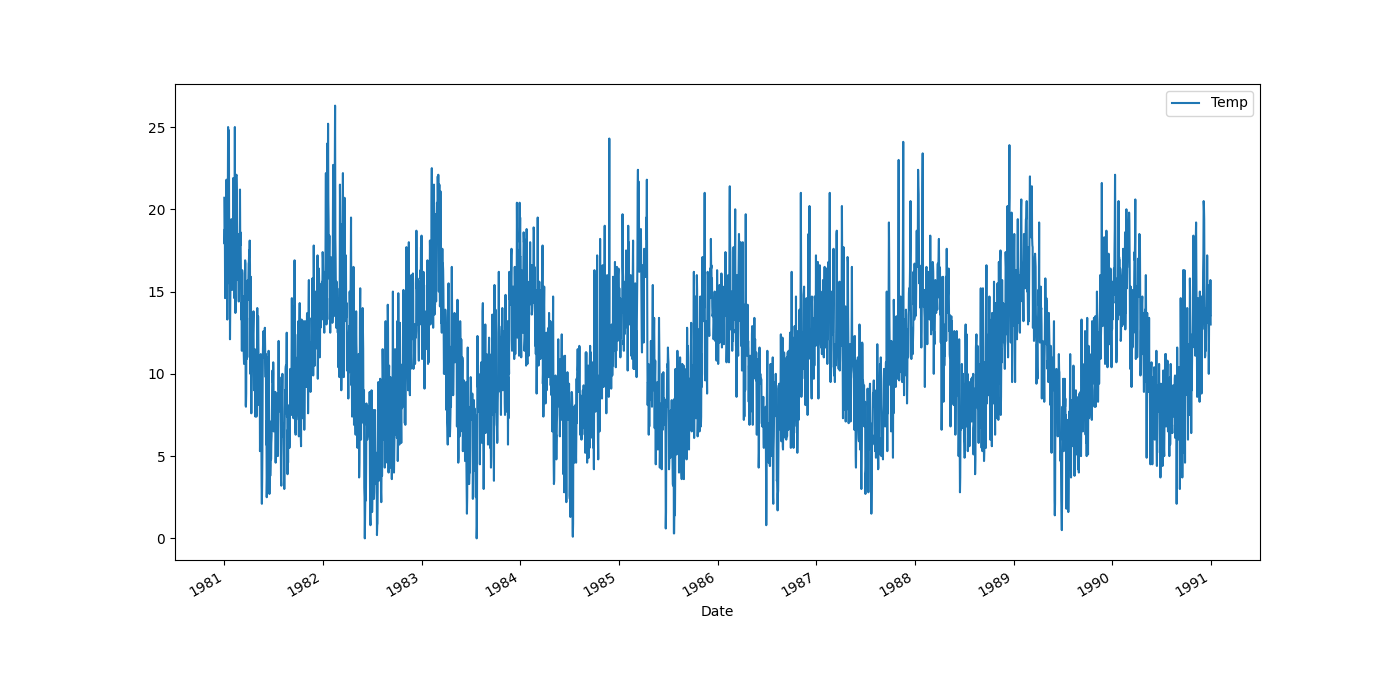
\includegraphics[width=\textwidth]{figures/Ass1/Ass1_D1_raw_signal.png}
    \end{minipage}
    \caption{Visualizing the raw signals of the first dataset.}
    \label{fig:Ass1_D1_raw_signal}
\end{figure}

\begin{figure}[H]
    \centering
    \begin{minipage}[b]{1\textwidth}
        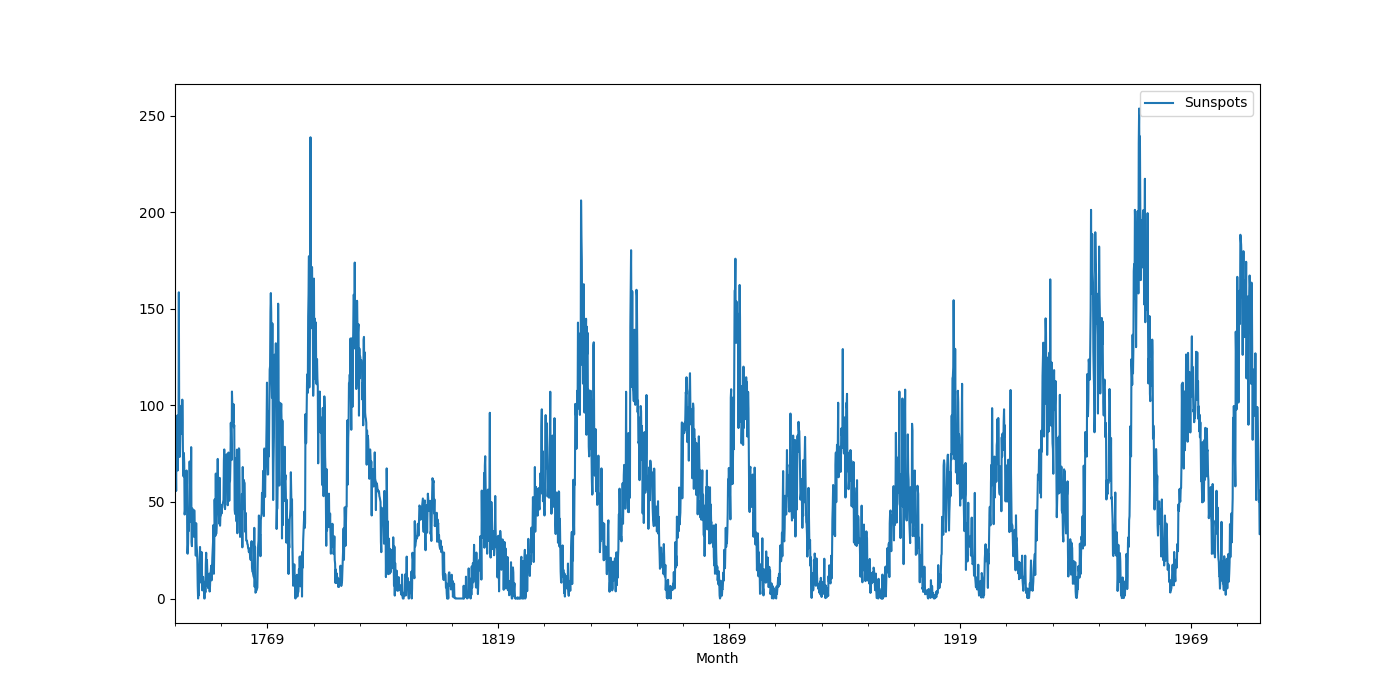
\includegraphics[width=\textwidth]{figures/Ass1/Ass1_D2_raw_signal.png}
    \end{minipage}
    \caption{Visualizing the raw signals of the second dataset.}
    \label{fig:Ass1_D2_raw_signal}
\end{figure}

\begin{figure}[H]
    \centering
    \begin{minipage}[b]{1\textwidth}
        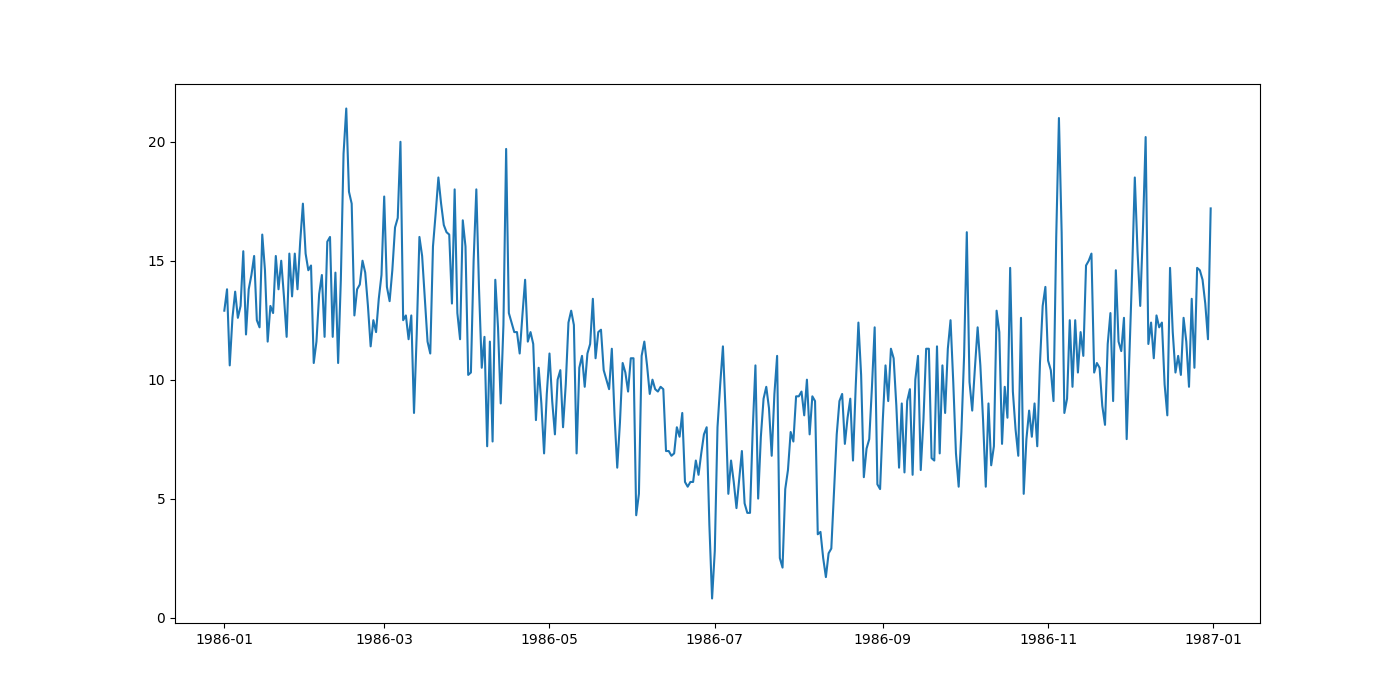
\includegraphics[width=\textwidth]{figures/Ass1/Ass1_D1_raw_signal_1986.png}
    \end{minipage}
    \caption{Visualizing the raw signals of the first dataset in 1986.}
    \label{fig:Ass1_D1_raw_signal_1986}
\end{figure}

\begin{figure}[H]
    \centering
    \begin{minipage}[b]{1\textwidth}
        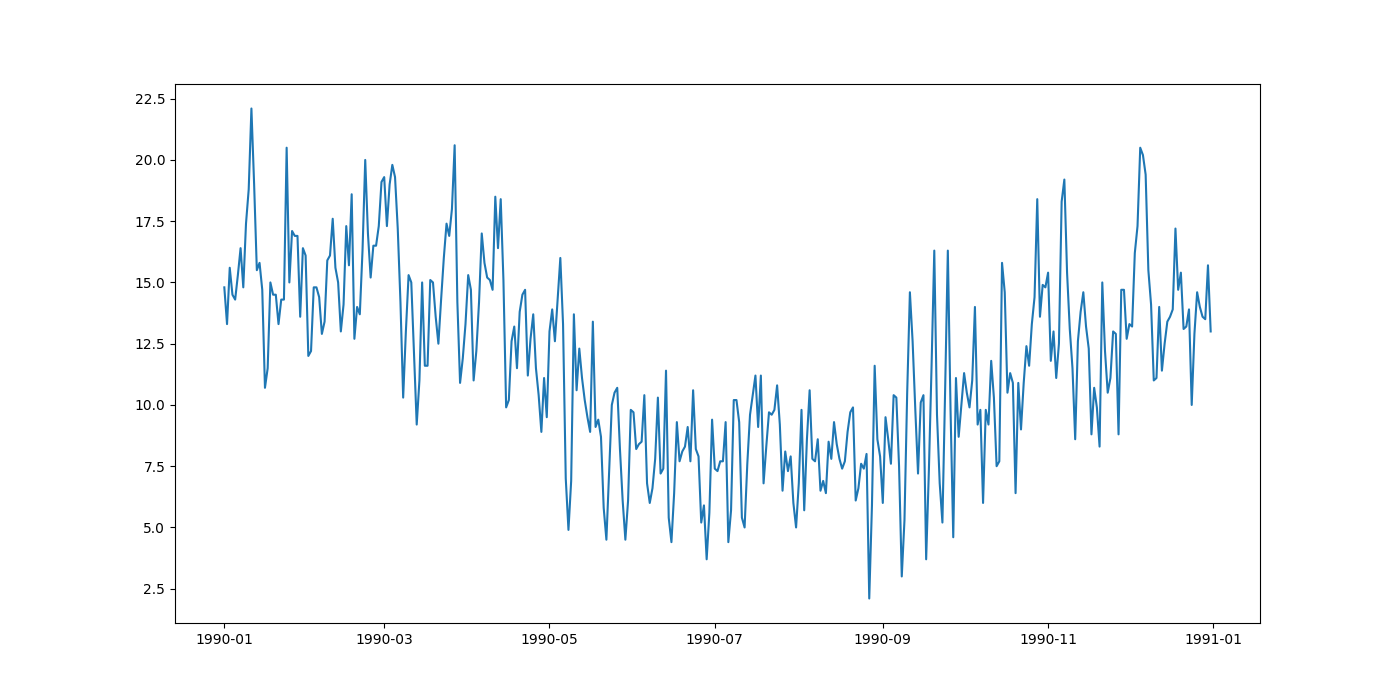
\includegraphics[width=\textwidth]{figures/Ass1/Ass1_D1_raw_signal_1990.png}
    \end{minipage}
    \caption{Visualizing the raw signals of the first dataset in 1990.}
    \label{fig:Ass1_D1_raw_signal_1990}
\end{figure}

\begin{figure}[H]
    \centering
    \begin{minipage}[b]{1\textwidth}
        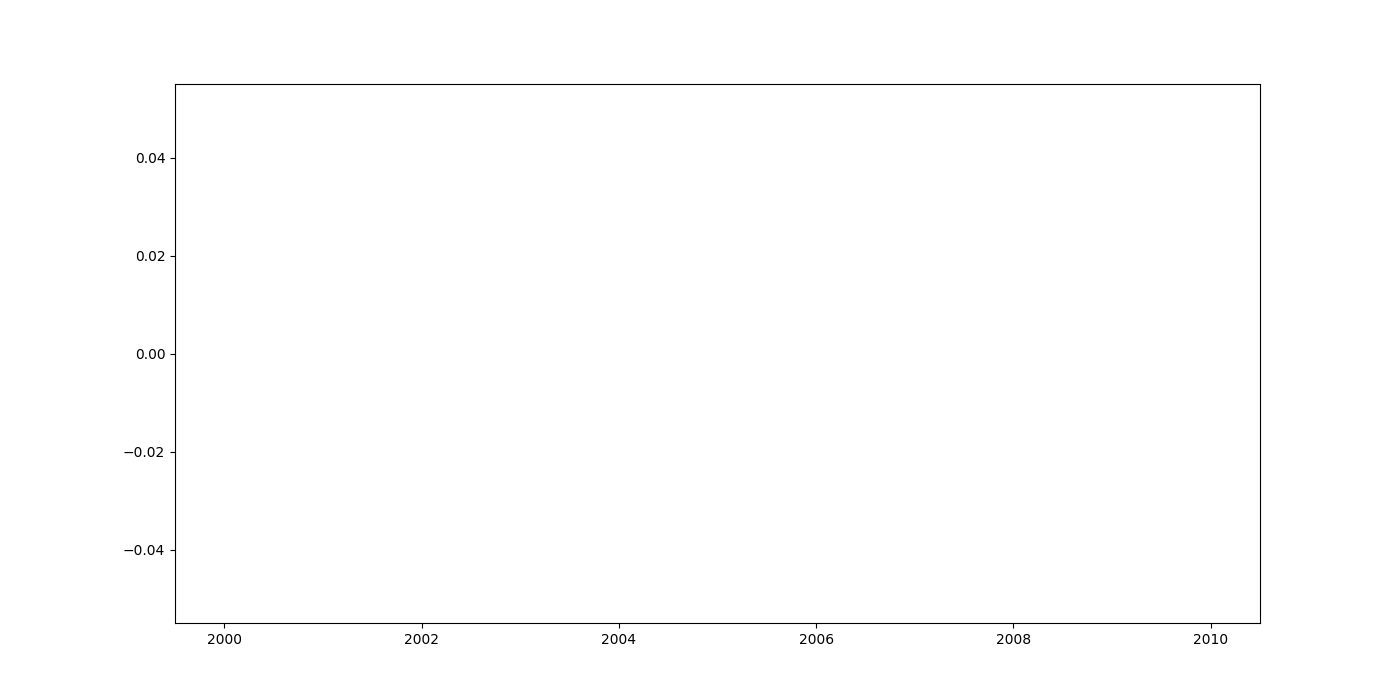
\includegraphics[width=\textwidth]{figures/Ass1/Ass1_D2_raw_signal_1990.png}
    \end{minipage}
    \caption{Visualizing the raw signals of the second dataset in 1990.}
    \label{fig:Ass1_D2_raw_signal_1990}
\end{figure}

\textit{For intuition, Table \ref{tab:Ass1_D1_raw_signal} to  \ref{tab:Ass1_D2_raw_signal_summary_statistics} show the top raw of two datasets along with the summary of two time series datasets.}


\begin{table}[H]
 \centering
\caption{The top row of the raw signal of the first dataset (daily temp).
{\label{tab:Ass1_D1_raw_signal}}}
\begin{tabular}{lr}
\toprule
{} &  Temp \\
Date       &       \\
\midrule
1981-01-01 &  20.7 \\
1981-01-02 &  17.9 \\
1981-01-03 &  18.8 \\
1981-01-04 &  14.6 \\
1981-01-05 &  15.8 \\
1981-01-06 &  15.8 \\
1981-01-07 &  15.8 \\
\bottomrule
\end{tabular}

\end{table}

\begin{table}[H]
 \centering
\caption{The description of the first dataset.
{\label{tab:Ass1_D1_raw_signal_summary_statistics}}}
\begin{tabular}{lr}
\toprule
{} &         Temp \\
\midrule
count &  3650.000000 \\
mean  &    11.177753 \\
std   &     4.071837 \\
min   &     0.000000 \\
25\%   &     8.300000 \\
50\%   &    11.000000 \\
75\%   &    14.000000 \\
max   &    26.300000 \\
\bottomrule
\end{tabular}

\end{table}

\begin{table}[H]
 \centering
\caption{The top row of the raw signal of the second dataset.
{\label{tab:Ass1_D2_raw_signal}}}
\begin{tabular}{lr}
\toprule
{} &  Sunspots \\
Month      &           \\
\midrule
1749-01-01 &      58.0 \\
1749-02-01 &      62.6 \\
1749-03-01 &      70.0 \\
1749-04-01 &      55.7 \\
1749-05-01 &      85.0 \\
\bottomrule
\end{tabular}

\end{table}

\begin{table}[H]
 \centering
\caption{The description of the second dataset.
{\label{tab:Ass1_D2_raw_signal_summary_statistics}}}
\begin{tabular}{lr}
\toprule
{} &     Sunspots \\
\midrule
count &  2820.000000 \\
mean  &    51.265957 \\
std   &    43.448971 \\
min   &     0.000000 \\
25\%   &    15.700000 \\
50\%   &    42.000000 \\
75\%   &    74.925000 \\
max   &   253.800000 \\
\bottomrule
\end{tabular}

\end{table}






\textit{For decomposing the data the below methods were used:}
    \begin{enumerate}
    \item \textit{Seasonal\_decompose (Figure
        \ref{fig:Ass1_D1_seasonal_decompose} and \ref{fig:Ass1_D2_seasonal_decompose})}
        
    \item \textit{STL (Figure
        \ref{fig:Ass1_D1_STL} and \ref{fig:Ass1_D2_STL})}
        
    \item \textit{Linear Regression method (Figure
        \ref{fig:Ass1_D1_LinearRegression_diff} and \ref{fig:Ass1_D2_LinearRegression_diff})}
        
    \item \textit{Difference method (Figure
        \ref{fig:Ass1_D1_one_diff} and \ref{fig:Ass1_D2_one_diff})}
        
    \item \textit{Fitting a polynomial (Figure
        \ref{fig:Ass1_D1_fiting_polynomial} and \ref{fig:Ass1_D2_fiting_polynomial})}
        
    \item \textit{Moving Average window (Figure
        \ref{fig:Ass1_D1_Moving_Avrage} and \ref{fig:Ass1_D2_Moving_Avrage})}

    \end{enumerate}
    
\textit{Some mentioned methods are used only for extracting only one component while others like STL and Seasonal\_decompose provided all three components. Table \ref{tab:Ass1_comparing_methods} compares these} methods together.

\textit{Also there are two model for reconstruction of time series, Additive Model and Multiplicative Model. In this assignment the additive model was used because Multiplicative is not appropriate for zero and negative values.}

\begin{table}[H]
\centering
\caption{Comparing the implemented methods.
\label{tab:Ass1_comparing_methods}}
\begin{tabular}{@{}lccc@{}}
\toprule
                    & \begin{tabular}[c]{@{}c@{}}Trend \\ component\end{tabular} & \begin{tabular}[c]{@{}c@{}}Seasonal \\ component\end{tabular} & \begin{tabular}[c]{@{}c@{}}Residual \\ component\end{tabular} \\ \midrule
Seasonal\_decompose & \checkmark                                  & \checkmark                                     & \checkmark                                     \\ \midrule
STL                 & \checkmark                                  & \checkmark                                     & \checkmark                                     \\ \midrule
Linear Regression   & \checkmark                                  & -                                                             & -                                                             \\ \midrule
Difference          & -                                                          & \checkmark                                     & -                                                             \\ \midrule
Moving average      & \checkmark                                  & -                                                             & -                                                             \\ \bottomrule
\end{tabular}

\end{table}




\begin{figure}[H]
    \centering
    \begin{minipage}[b]{1\textwidth}
        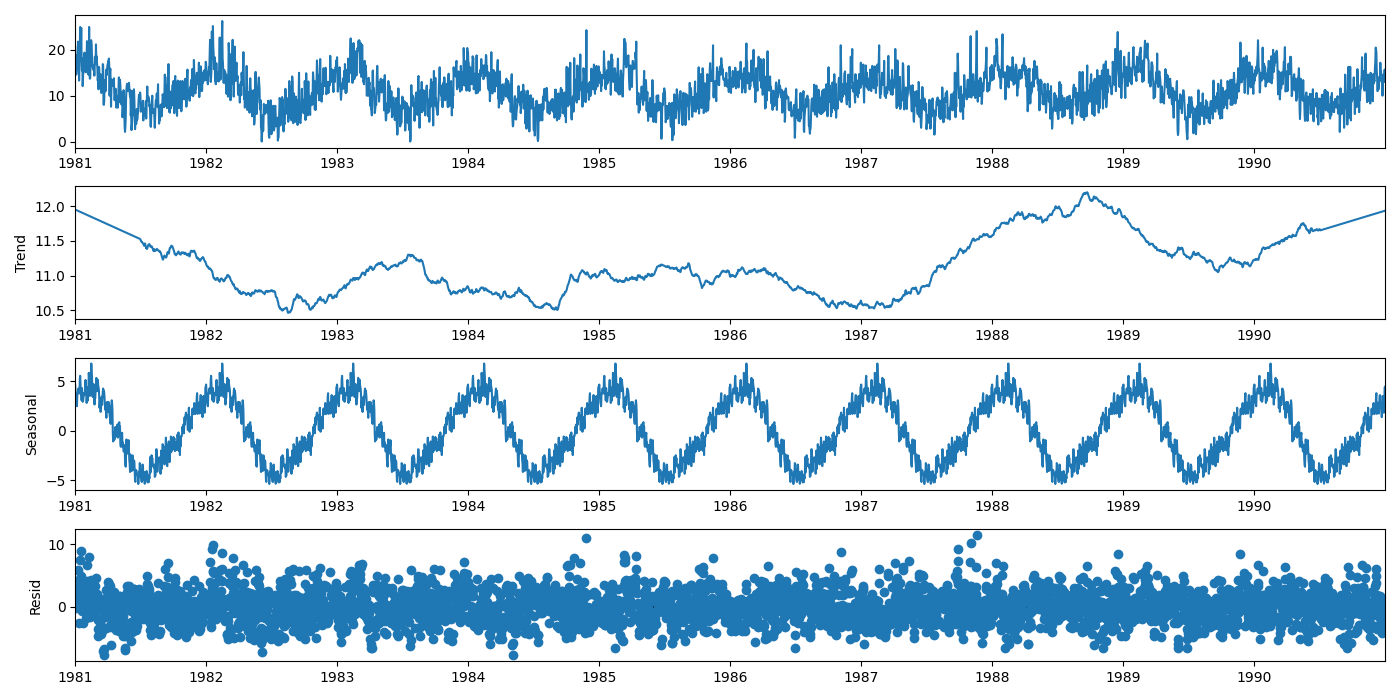
\includegraphics[width=\textwidth]{figures/Ass1/Ass1_D1_seasonal_decompose.png}
    \end{minipage}
    \caption{Decomposition of the first dataset by seasonal\_decompose method}
    \label{fig:Ass1_D1_seasonal_decompose}
\end{figure}

\begin{figure}[H]
    \centering
    \begin{minipage}[b]{1\textwidth}
        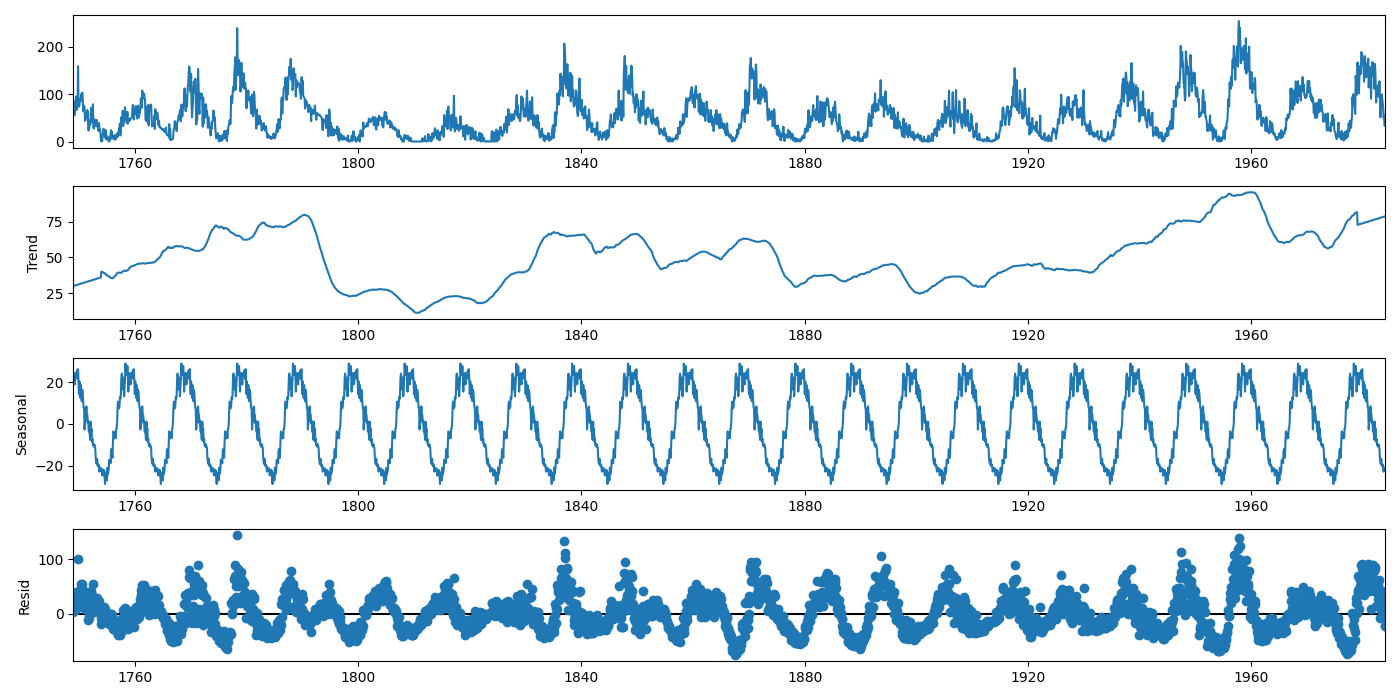
\includegraphics[width=\textwidth]{figures/Ass1/Ass1_D2_seasonal_decompose.png}
    \end{minipage}
    \caption{Decomposition of the second dataset by seasonal\_decompose method}
    \label{fig:Ass1_D2_seasonal_decompose}
\end{figure}

\begin{figure}[H]
    \centering
    \begin{minipage}[b]{1\textwidth}
        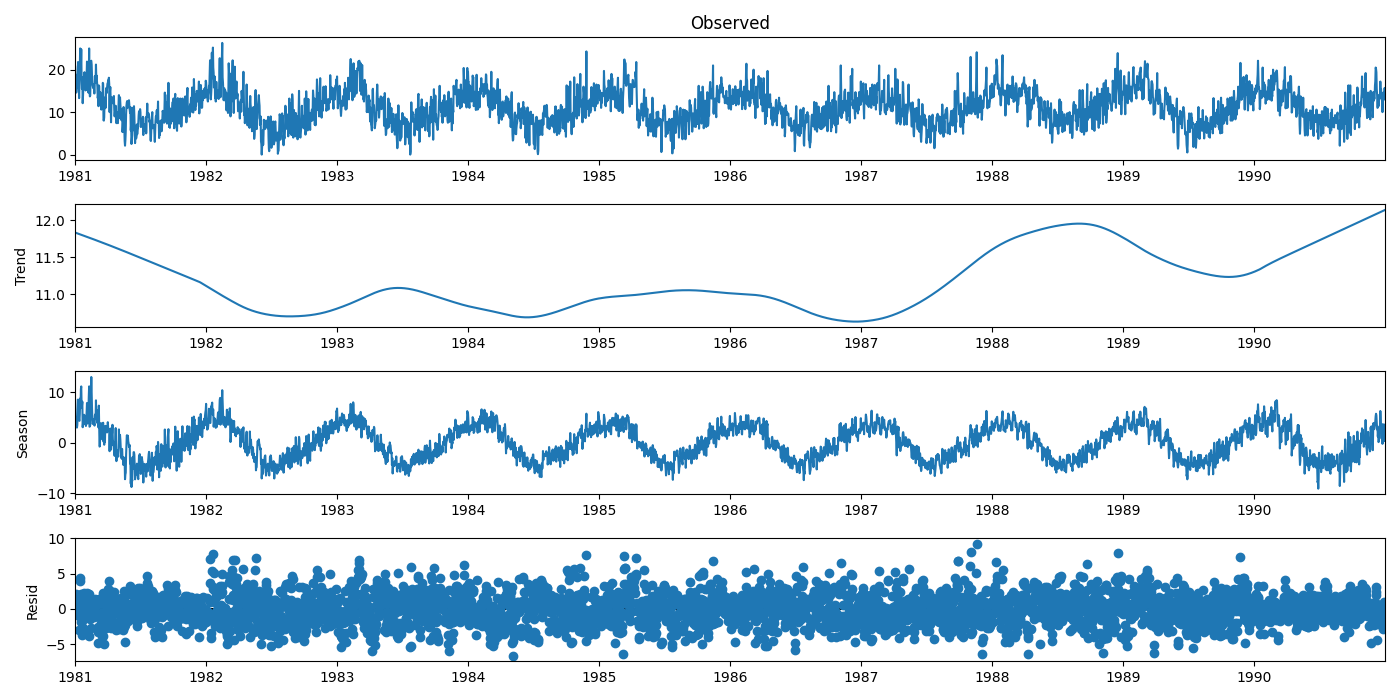
\includegraphics[width=\textwidth]{figures/Ass1/Ass1_D1_STL.png}
    \end{minipage}
    \caption{Decomposition of the first dataset by STL method}
    \label{fig:Ass1_D1_STL}
\end{figure}

\begin{figure}[H]
    \centering
    \begin{minipage}[b]{1\textwidth}
        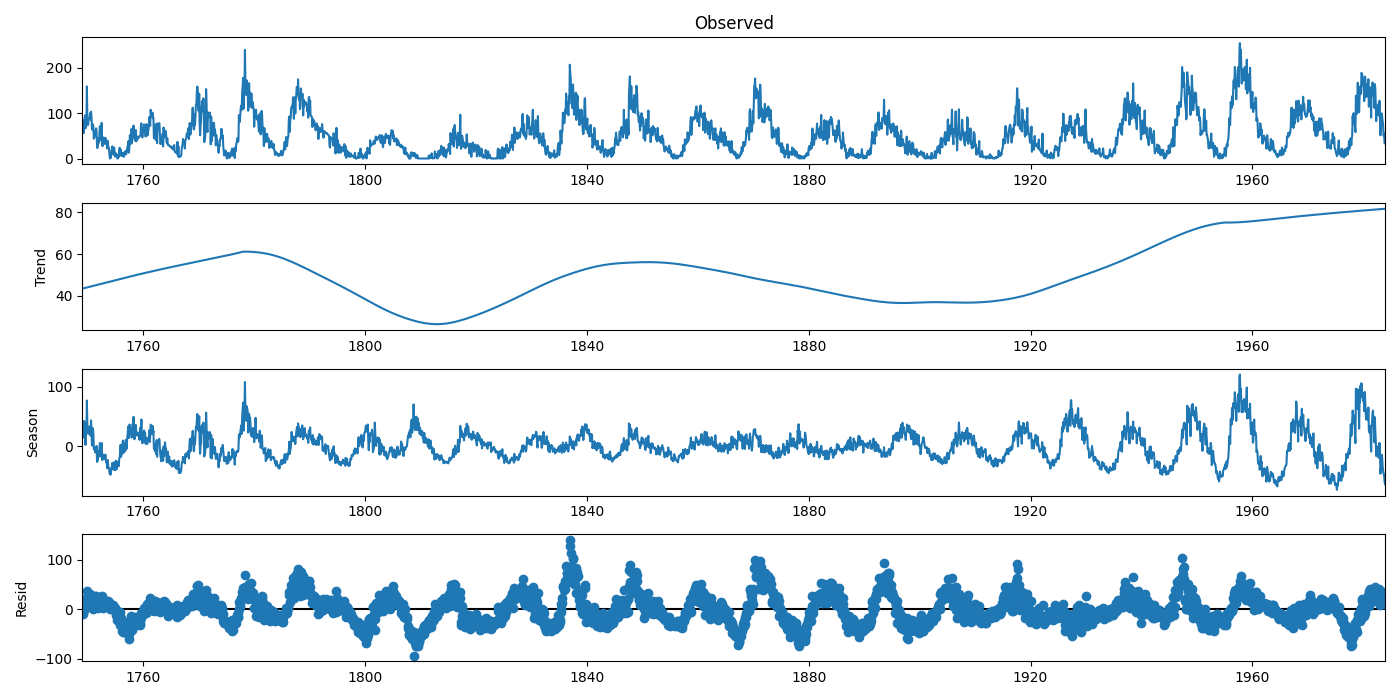
\includegraphics[width=\textwidth]{figures/Ass1/Ass1_D2_STL.png}
    \end{minipage}
    \caption{Decomposition of the second dataset by STL method}
    \label{fig:Ass1_D2_STL}
\end{figure}

\begin{figure}[H]
    \centering
    \begin{minipage}[b]{1\textwidth}
        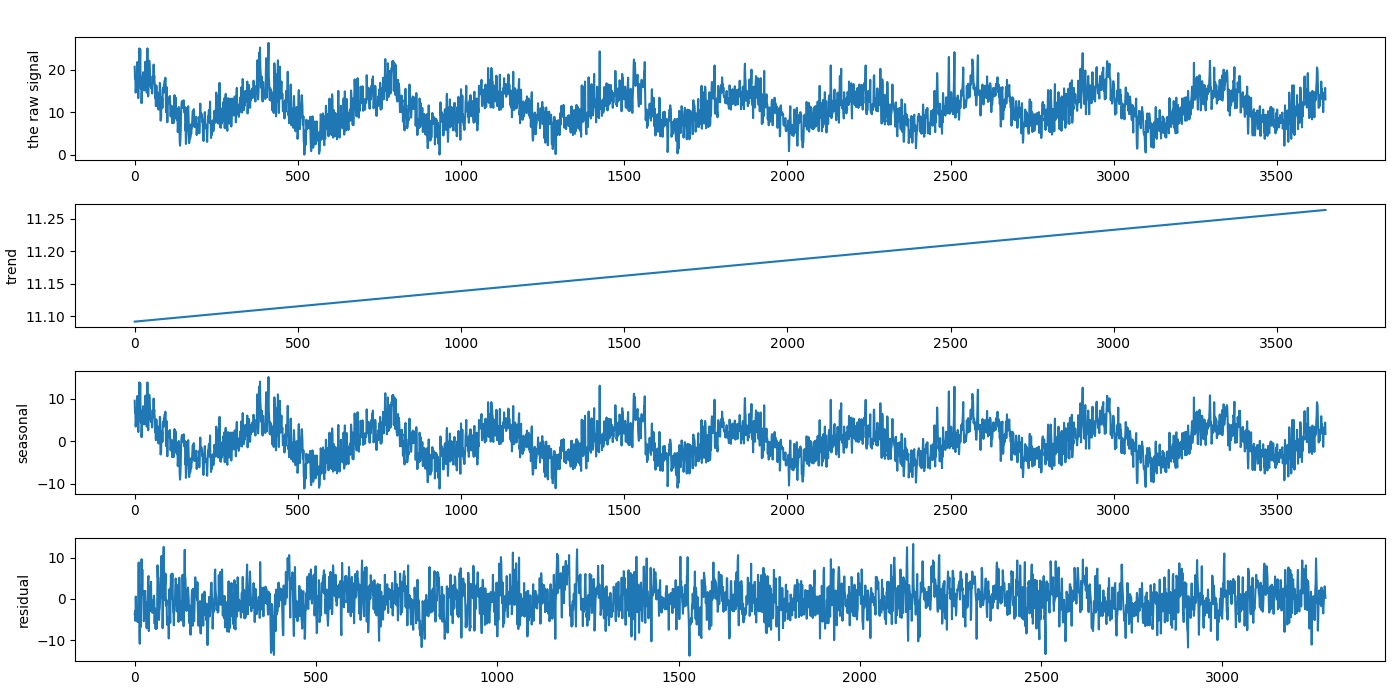
\includegraphics[width=\textwidth]{figures/Ass1/Ass1_D1_LinearRegression_diff.png}
    \end{minipage}
    \caption{Decomposition of the first dataset by LinearRegression and difference method.}
    \label{fig:Ass1_D1_LinearRegression_diff}
\end{figure}

\begin{figure}[H]
    \centering
    \begin{minipage}[b]{1\textwidth}
        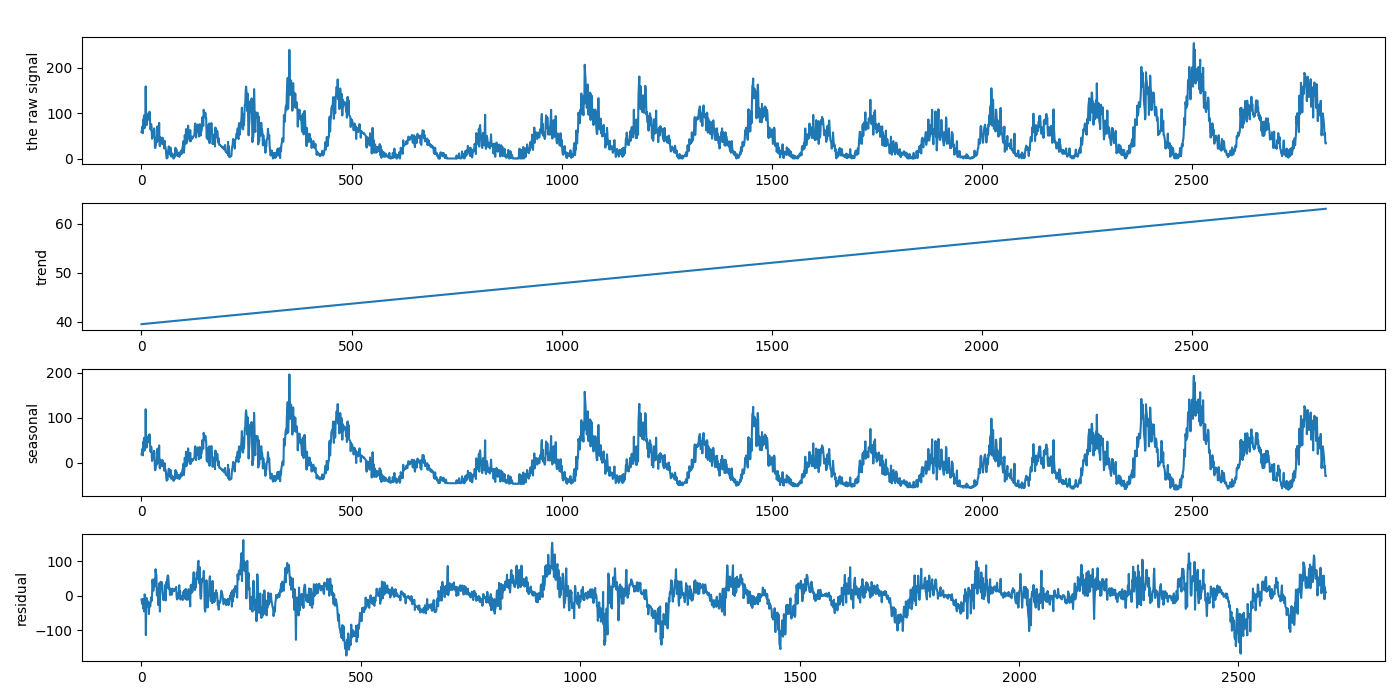
\includegraphics[width=\textwidth]{figures/Ass1/Ass1_D2_LinearRegression_diff.png}
    \end{minipage}
    \caption{Decomposition of the second dataset by LinearRegression and difference method.}
    \label{fig:Ass1_D2_LinearRegression_diff}
\end{figure}

\begin{figure}[H]
    \centering
    \begin{minipage}[b]{1\textwidth}
        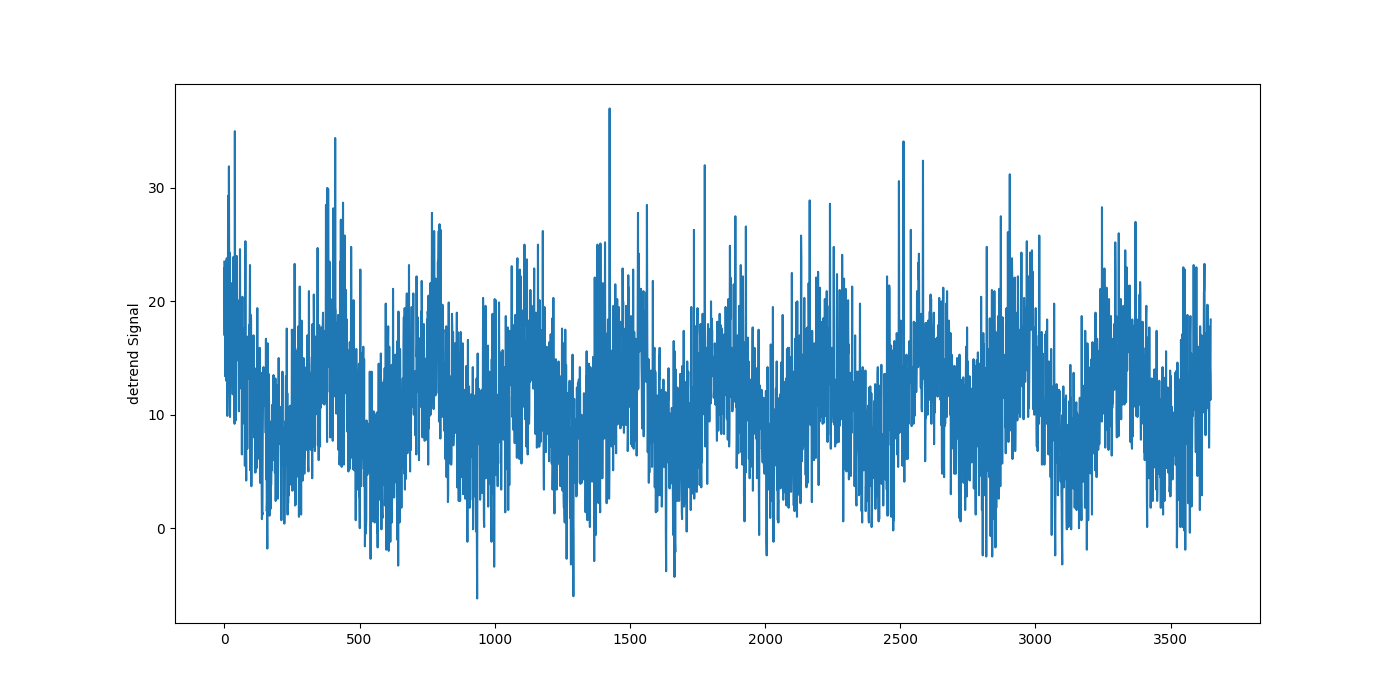
\includegraphics[width=\textwidth]{figures/Ass1/Ass1_D1_one_diff.png}
    \end{minipage}
    \caption{Detrending of the first dataset by difference method.}
    \label{fig:Ass1_D1_one_diff}
\end{figure}

\begin{figure}[H]
    \centering
    \begin{minipage}[b]{1\textwidth}
        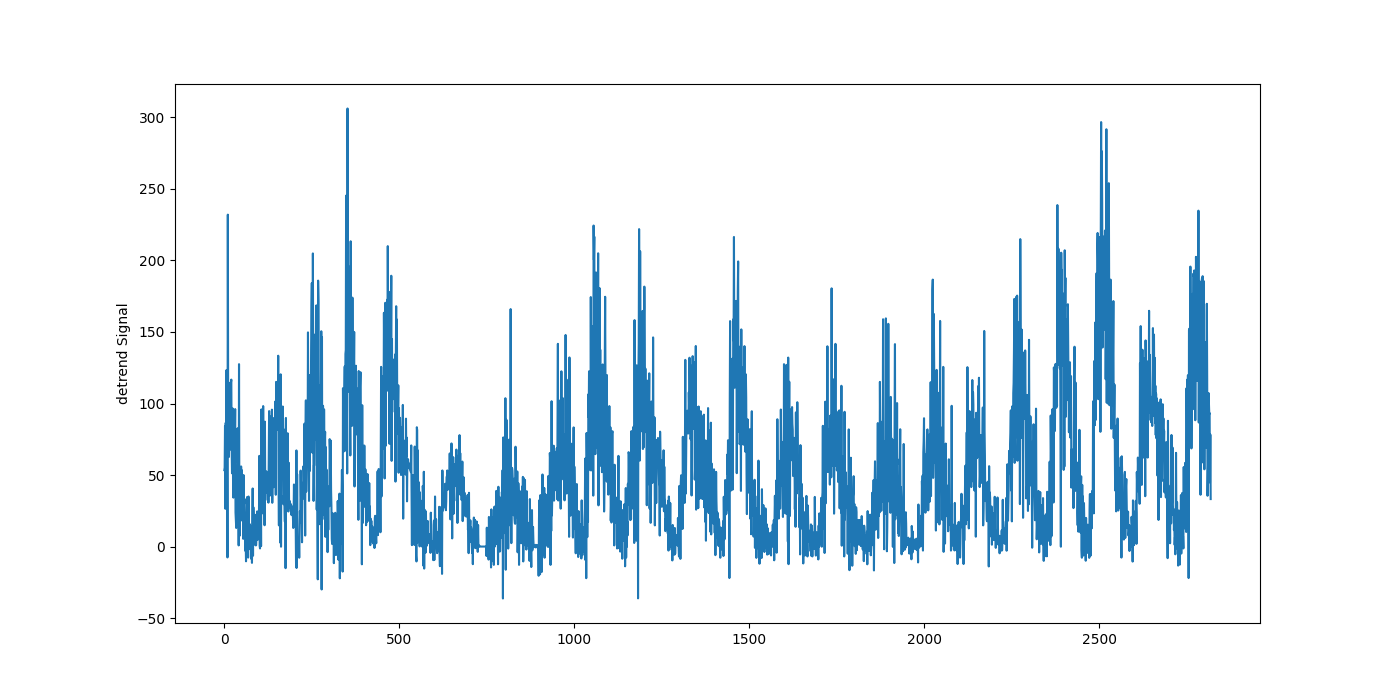
\includegraphics[width=\textwidth]{figures/Ass1/Ass1_D2_one_diff.png}
    \end{minipage}
    \caption{Detrending of the second dataset by difference method.}
    \label{fig:Ass1_D2_one_diff}
\end{figure}

\begin{figure}[H]
    \centering
    \begin{minipage}[b]{1\textwidth}
        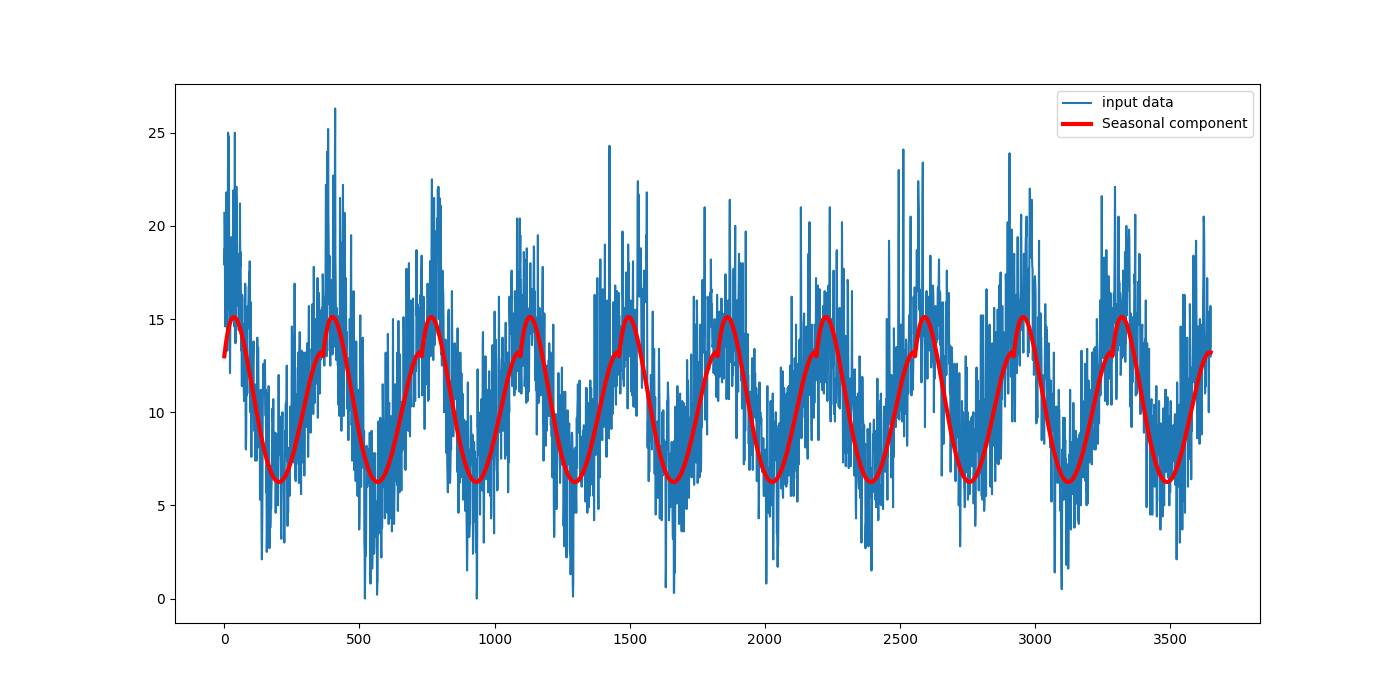
\includegraphics[width=\textwidth]{figures/Ass1/Ass1_D1_fiting_polynomial.png}
    \end{minipage}
    \caption{Seasonal component of the first dataset by fitting a polynomial.}
    \label{fig:Ass1_D1_fiting_polynomial}
\end{figure}

\begin{figure}[H]
    \centering
    \begin{minipage}[b]{1\textwidth}
        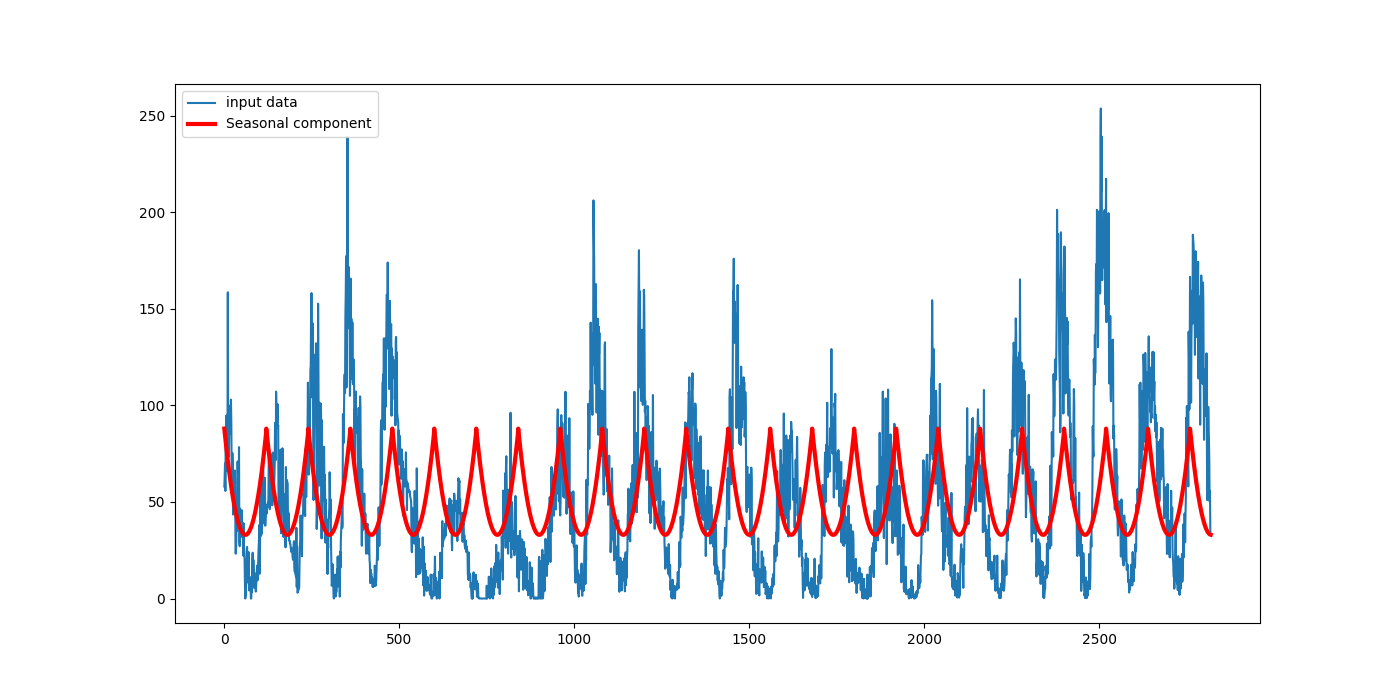
\includegraphics[width=\textwidth]{figures/Ass1/Ass1_D2_fiting_polynomial.png}
    \end{minipage}
    \caption{Seasonal component of the second dataset by fitting a polynomial.}
    \label{fig:Ass1_D2_fiting_polynomial}
\end{figure}

\begin{figure}[H]
    \centering
    \begin{minipage}[b]{1\textwidth}
        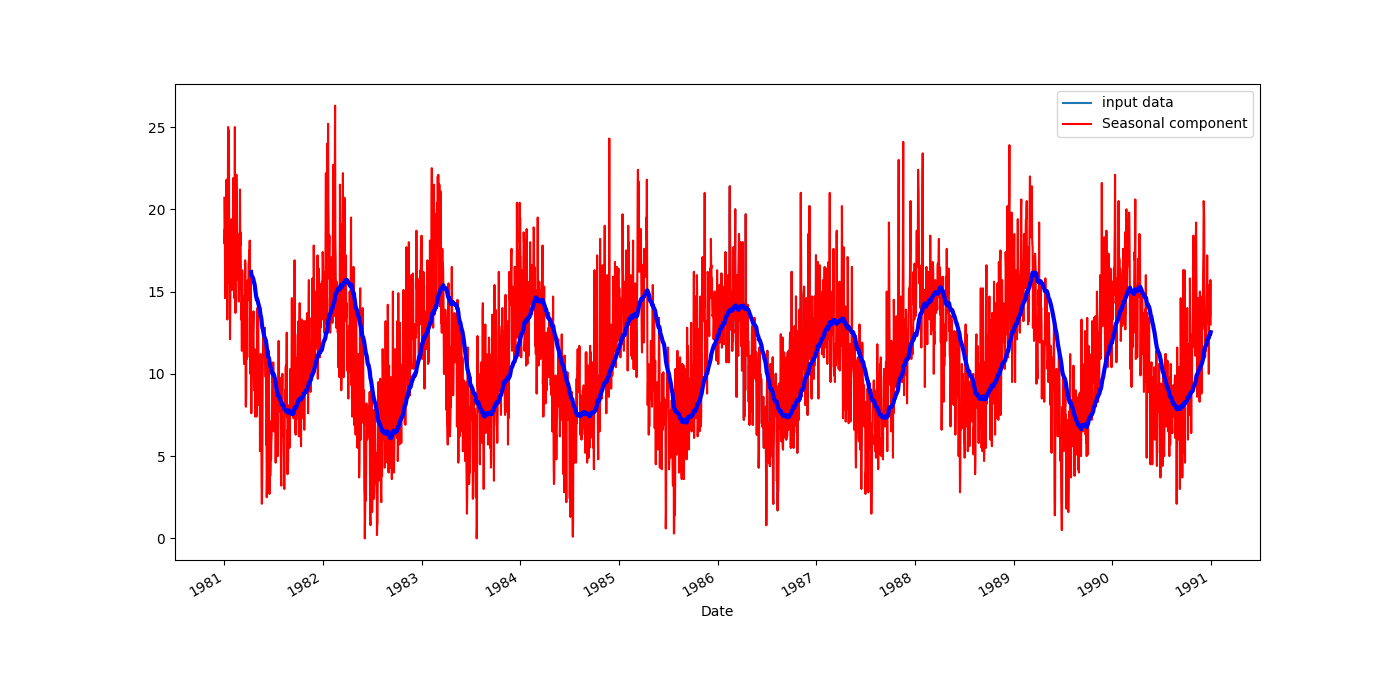
\includegraphics[width=\textwidth]{figures/Ass1/Ass1_D1_Moving_Avrage.png}
    \end{minipage}
    \caption{Seasonal component of the first dataset by Moving Average.}
    \label{fig:Ass1_D1_Moving_Avrage}
\end{figure}

\begin{figure}[H]
    \centering
    \begin{minipage}[b]{1\textwidth}
        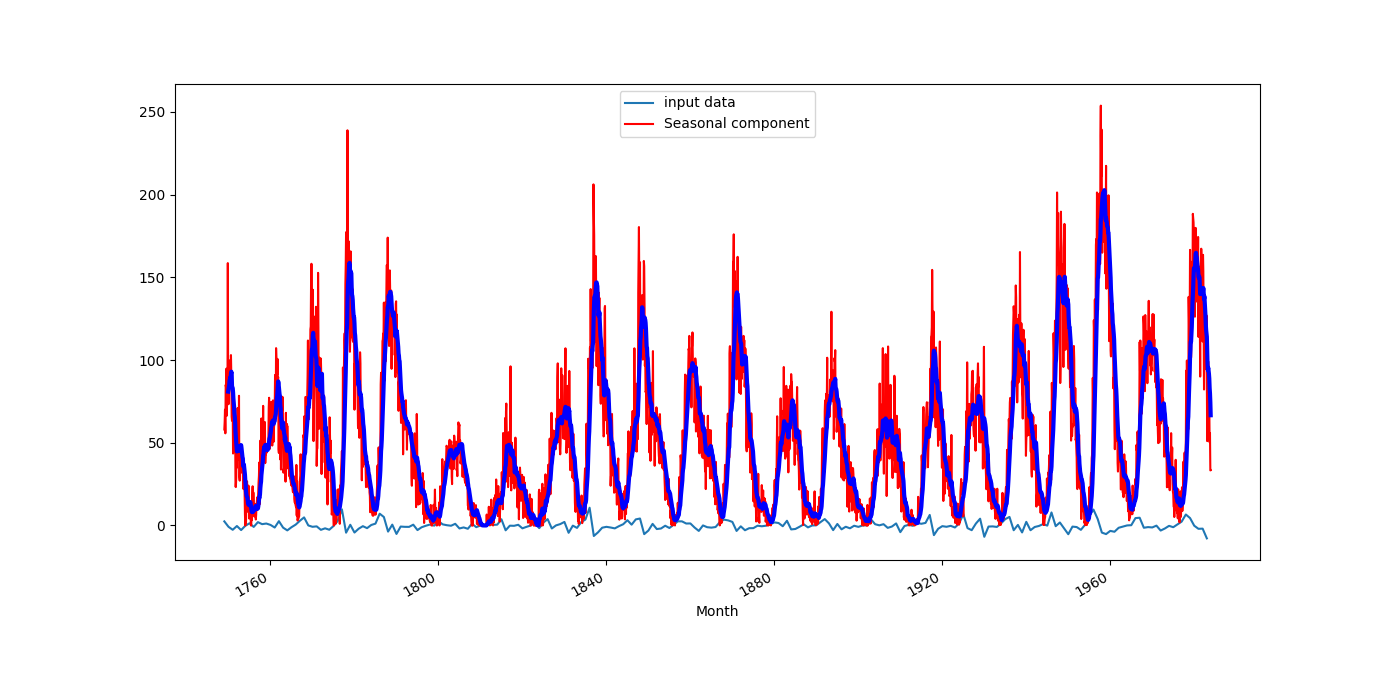
\includegraphics[width=\textwidth]{figures/Ass1/Ass1_D2_Moving_Avrage.png}
    \end{minipage}
    \caption{Seasonal component of the second dataset by Moving Average.}
    \label{fig:Ass1_D2_Moving_Avrage}
\end{figure}
